\setlength{\parskip}{\baselineskip}
\section[FL architecture]{FL architecture \& design}

\begin{frame}
	\huge FL architecture \& design
\end{frame}

\begin{frame}{Process \& Memory Layout}
	\begin{minipage}{0.4\textwidth}
        \begin{figure}[H]
            \centering
                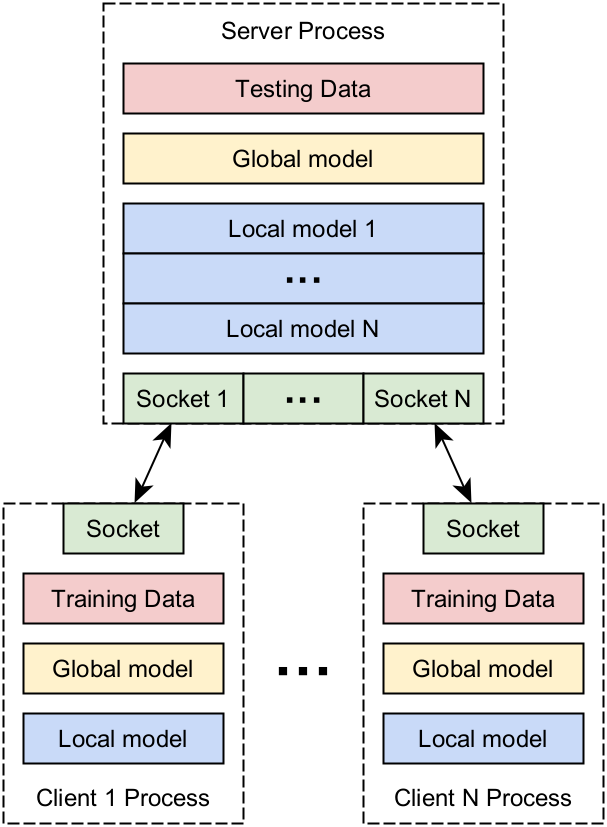
\includegraphics[height=0.8\textheight]{Images/Diagrams/memory_layout.png}
                % \caption{Process \& Memory layout of the developed FL system.}
        \end{figure}
    \end{minipage}%
	\begin{minipage}{0.6\textwidth}
	    Each entity is a distinct process with its own memory space.\\\\
	    POSIX sockets with TCP protocol.\\\\
	    TCP segments large messages, server have to keep copies of all models.
    \end{minipage}
\end{frame}

\begin{frame}{Communication Scheme}
    % Minimize the size of the communication
	\begin{table}[H]
        \center
        \begin{tabular}{ | c | }
            \hline
            Server to client message\\
            \hline\hline
            flags\\
            \hline
            GE\\
            \hline
            global model variables\\
            ...\\
            \hline
            \multicolumn{1}{ c }{ } \\
        \end{tabular}
        \quad
        \begin{tabular}{ | c | }
            \hline
            Client to server message\\
            \hline\hline
            GE\\
            \hline
            local loss\\
            \hline
            local accuracy\\
            \hline
            model variables / deltas\\
            ...\\
            \hline
        \end{tabular}
        \caption[Communication Scheme]{The format of the communication between the server and the clients.}
    \end{table}
\end{frame}

% \begin{frame}{Server}
%     The server adheres to the Event-driven server paradigm. After necessary initializations, it sleeps until one of the following events is raised:\\
%     \begin{itemize}
%         \item a client is trying to connect
%         \item a connected socket receives data
%         \item a connected socket can send data
%         \item a connected socket encounters an error
%     \end{itemize}
%     All events are non-blocking! Multiple events are required to receive or send data.
    
%     After every event, it checks if the next GE is ready. If it is, it creates the next global model and select connections to participate in next epoch.
% \end{frame}

% \begin{frame}{Client}
%     After necessary initializations, the client tries to connect to the server. If accepted, it operates as follows:\\
%     \begin{itemize}
%         \item waits to receive a global model
%         \item calculates a new local model using the global model \& its private data
%         \item sends its local model to the server
%     \end{itemize}
%     All communication is blocking, and controls the operation of the client.
% \end{frame}

\begin{frame}{Synchronization}
	\begin{minipage}{0.4\textwidth}
        \begin{figure}[H]
            \centering
                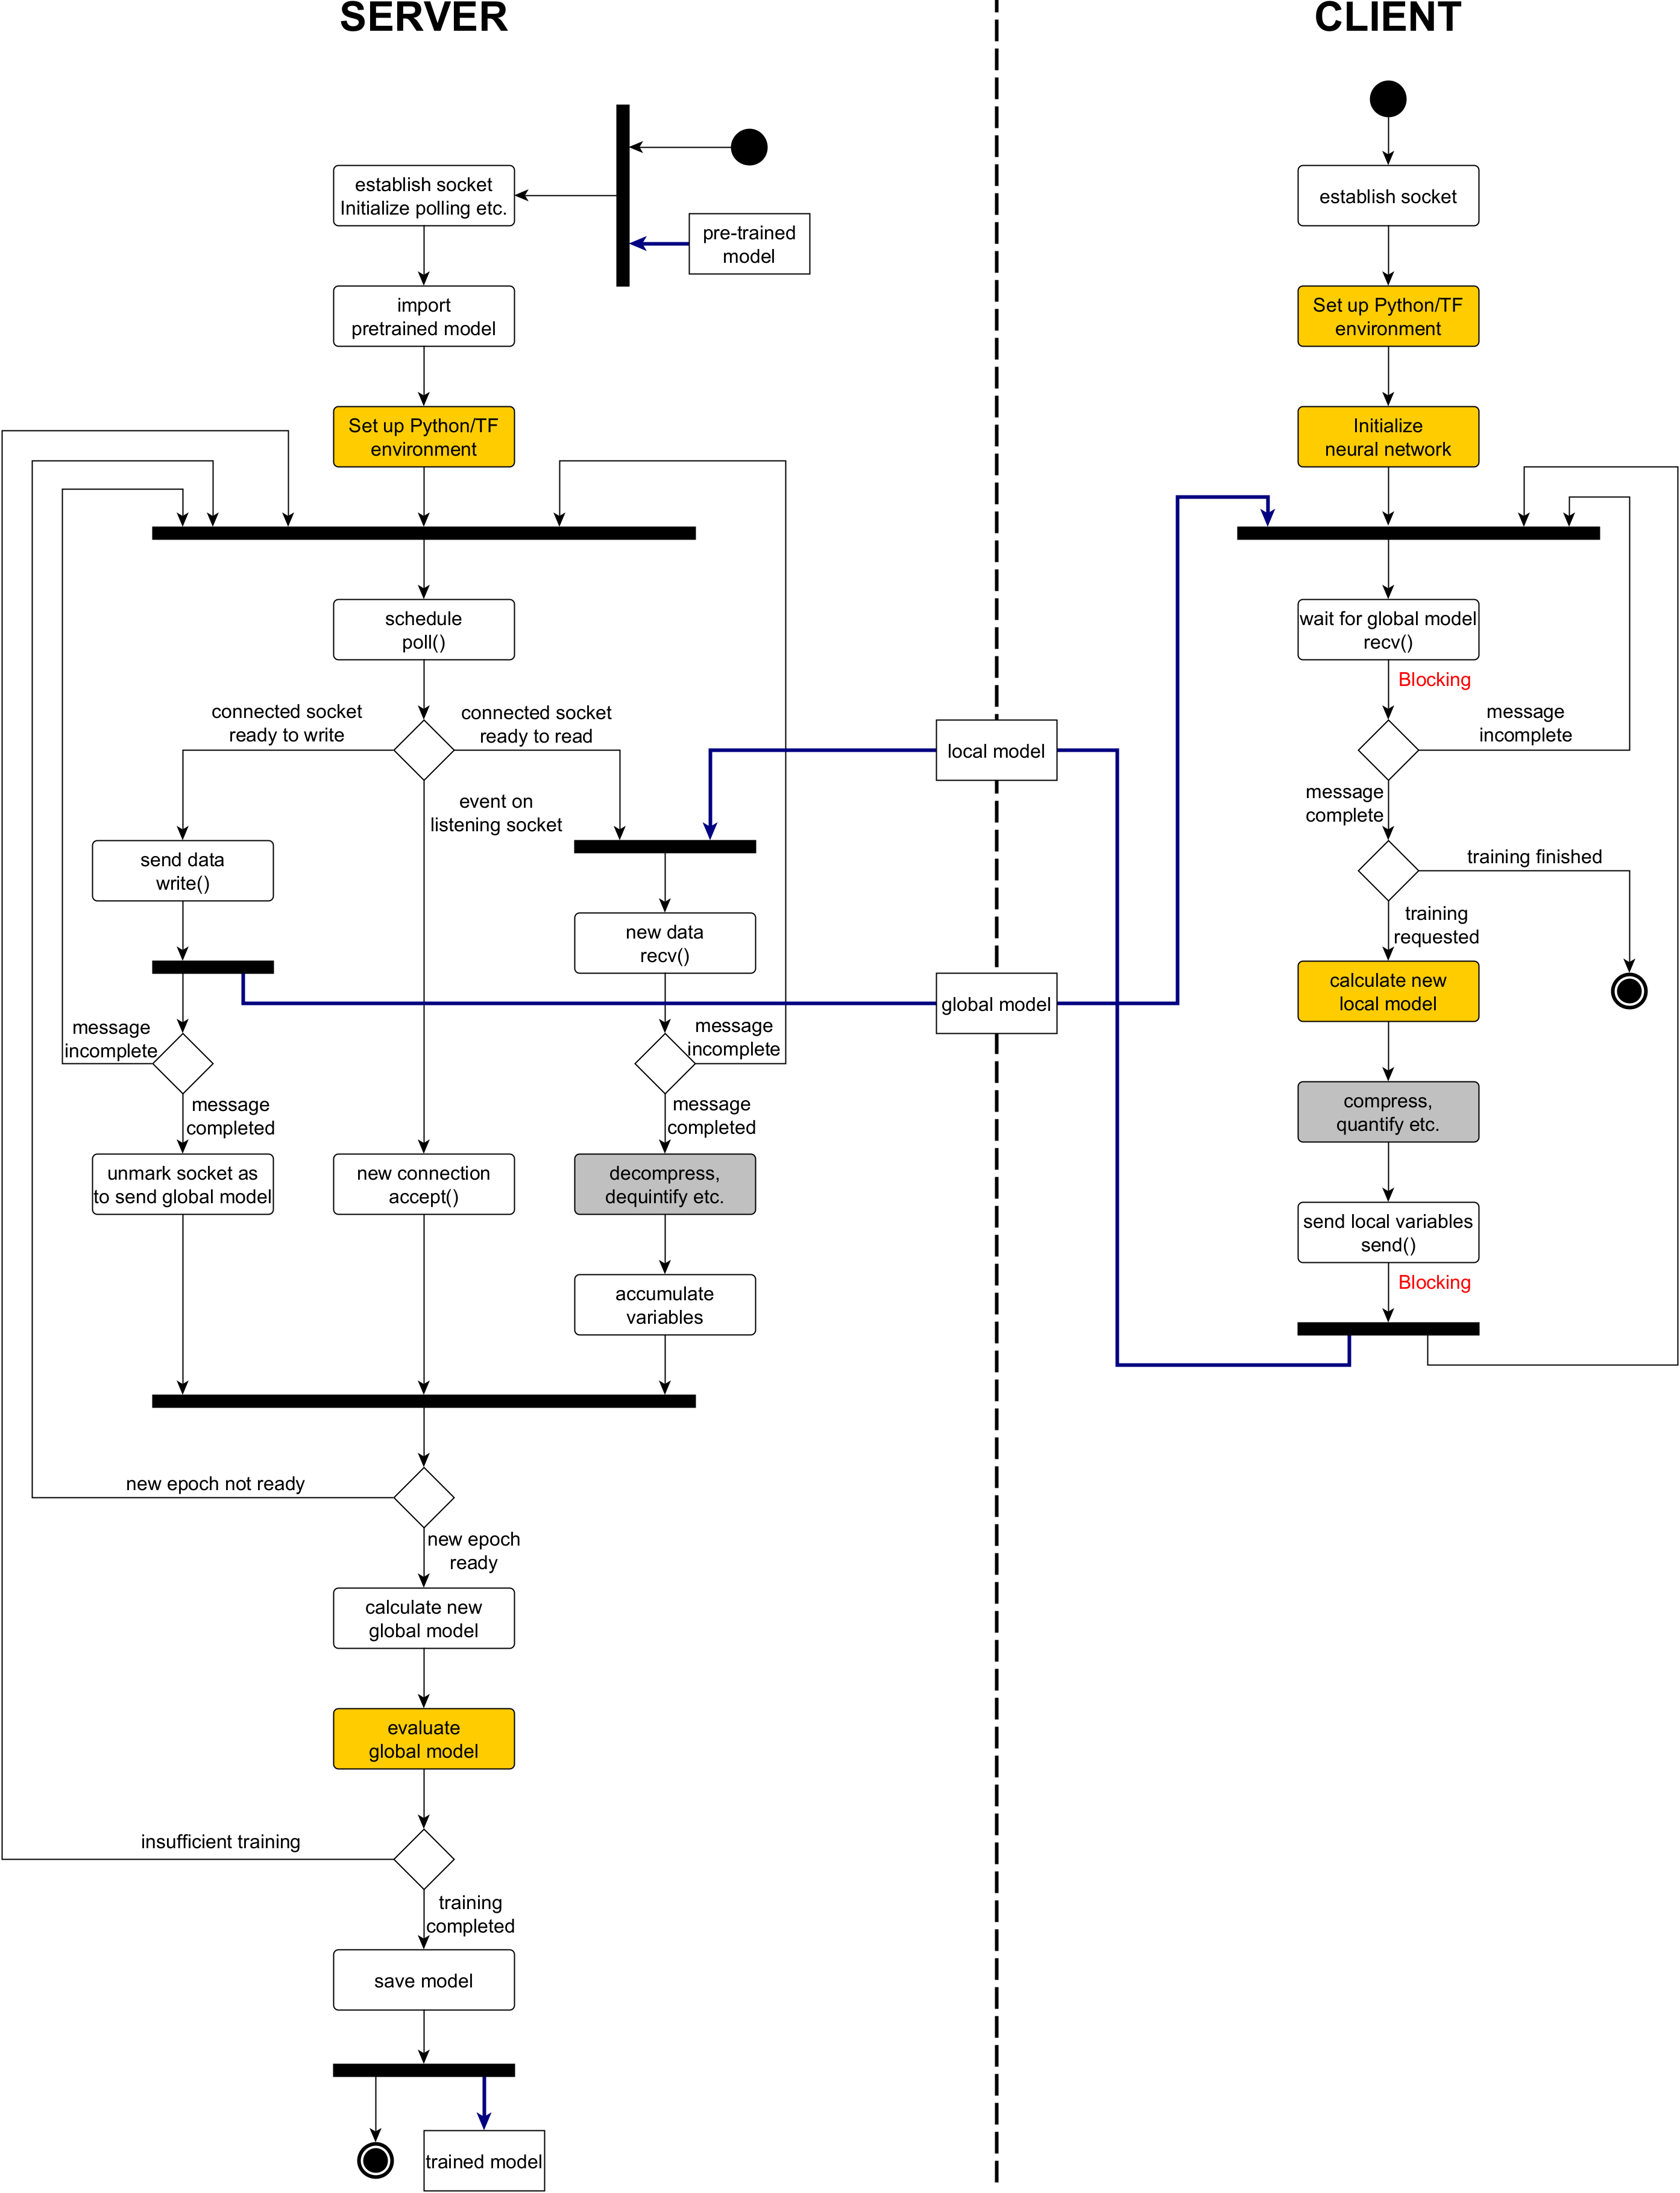
\includegraphics[height=0.85\textheight]{Images/Diagrams/top.png}
        \end{figure}
    \end{minipage}%
	\begin{minipage}{0.6\textwidth}
	    Event-driven server paradigm.\\\\
	    Large messages, multiple events are required to send \& receive them.\\\\
        Typical master-slave relationship between the server and the client.\\\\
        Multiple clients are connected to the server.\\\\
        Connectivity issues with a client, do not affect the communication with the rest.
    \end{minipage}
\end{frame}


% \begin{frame}{Embedding the Python Interpreter}
%     \onslide<1->
%     The FL system is developed in C++. To enable quick prototyping, the Python API of Tensorflow is used. 
    
%     \textbf{Problem:} Connecting these two parts is non-trivial.
    
%     \onslide<2->
%     \textbf{Solution:} Use the C/Python API to embed the Python Interpreter in the compiled process.\\
%     \begin{itemize}
%         \item C++ code can call Python functions
%         \item Python code can access C++ data by reference, using NumPy metadata
%     \end{itemize}\\
%     Low-level API, boilerplate code required to utilize it effectively.
% \end{frame}

% \begin{frame}{Embedding the Python Interpreter}
%     \begin{figure}[H]
%         \centering
%         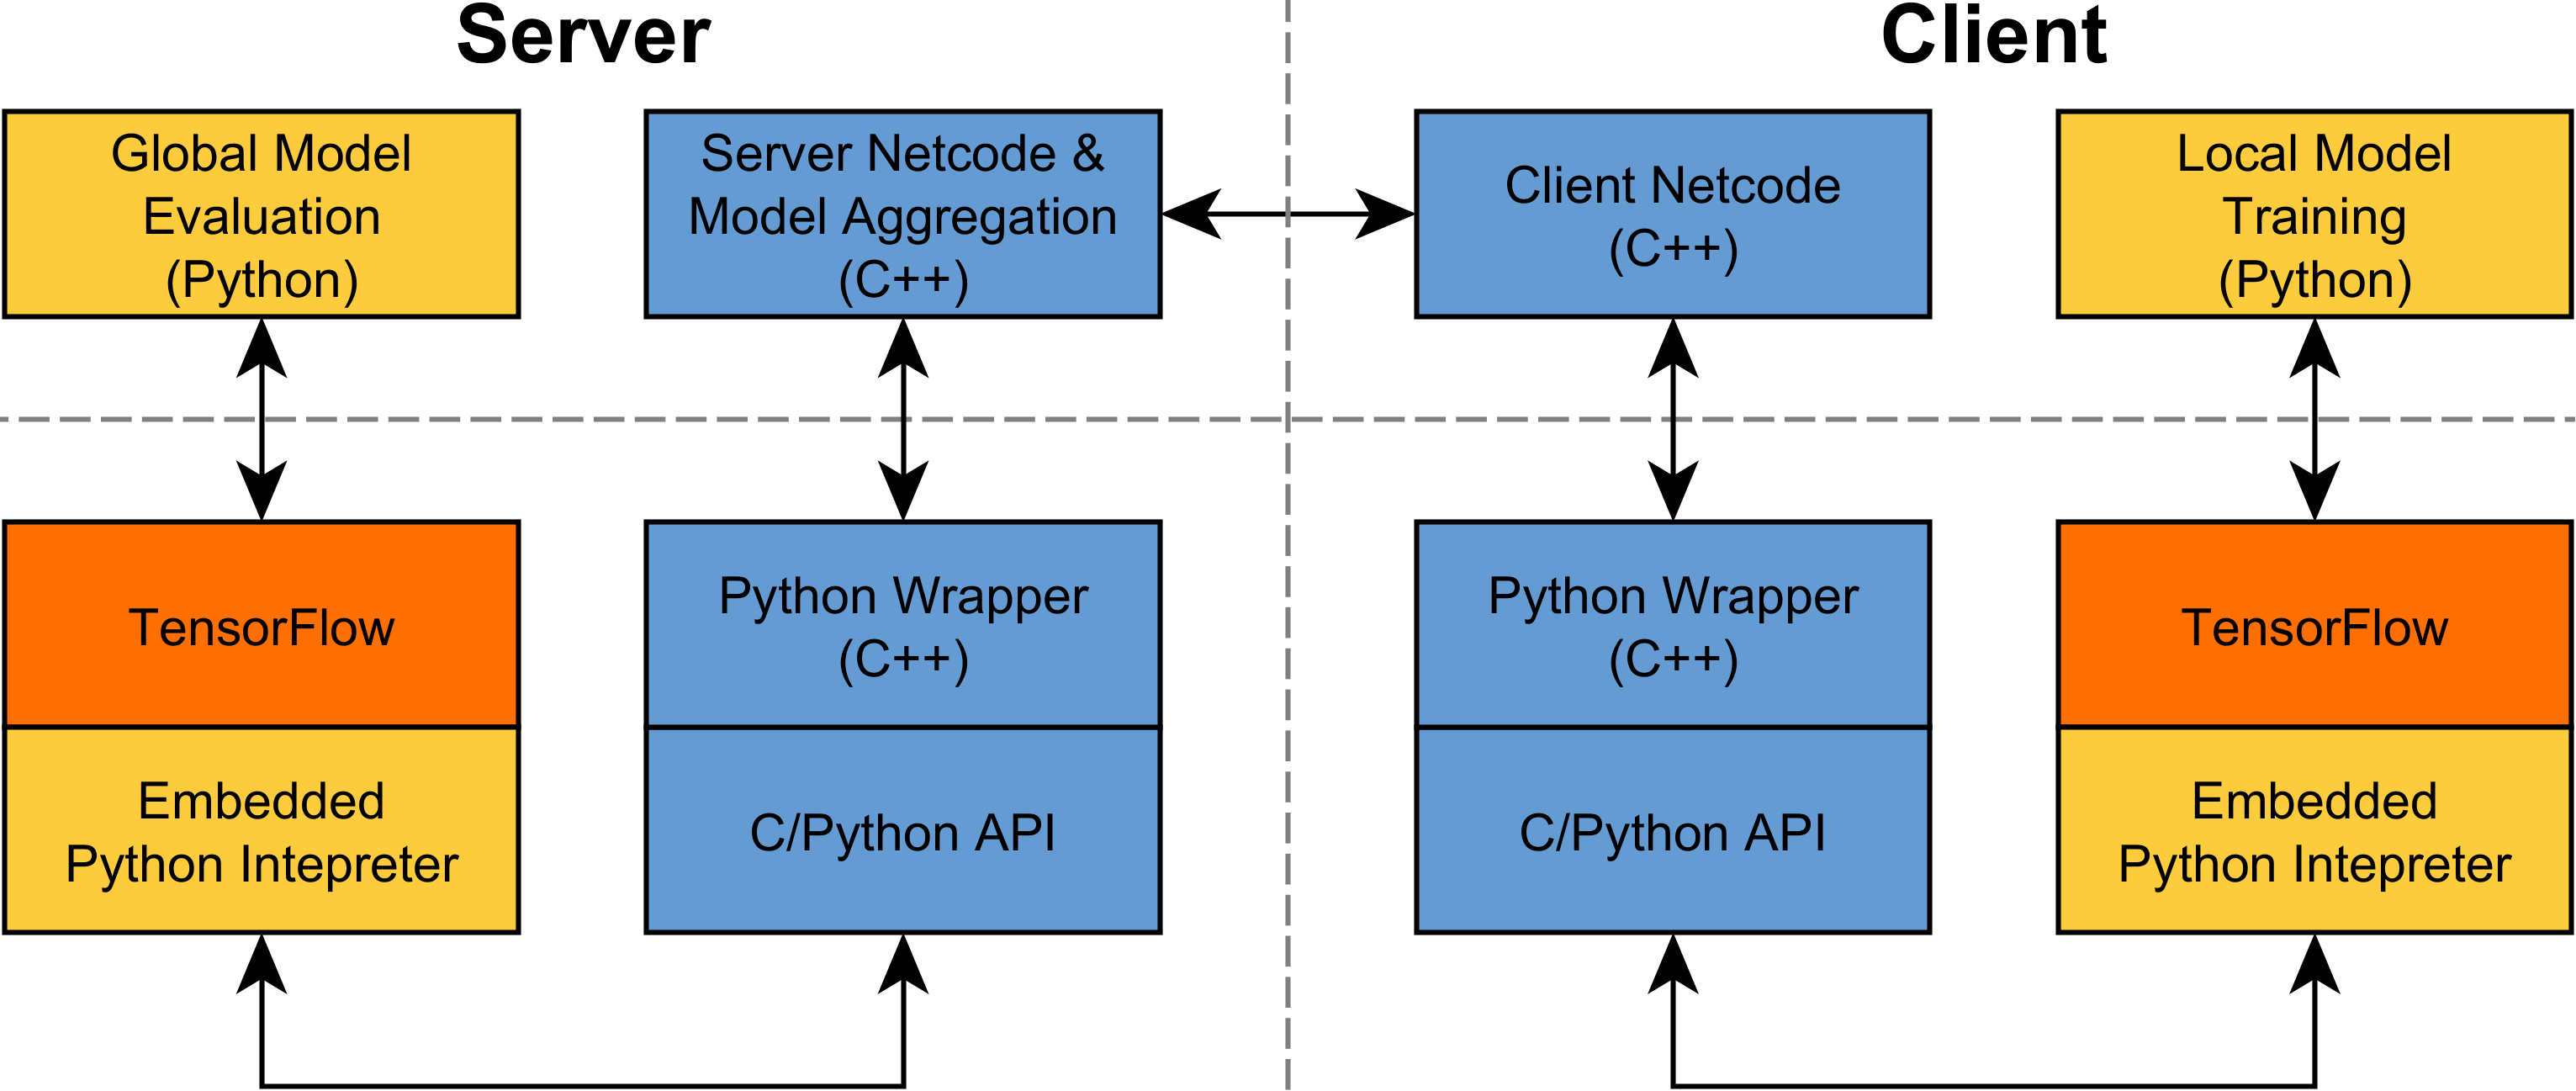
\includegraphics[width=0.75\textwidth]{Images/Diagrams/model_lifecycle.png}
%         \caption[]{Blue: C++ / Yellow, orange: Python, TF}
%     \end{figure}
% \end{frame}


\begin{frame}{Model Library}
    TensorFlow is incorporated to test the developed FL system.
    
    10 models used, including:\\
    \begin{itemize}
        \item DNNs
        \item CNNs
        \item based on the Inception Module
        \item RNNs
    \end{itemize}
    Most models are using ReLU and Softmax activations. Their sizes range between 60 thousand to 60 million parameters.
\end{frame}

% \begin{frame}{Data Preparation}
%     Preprocess and pre-distribute the dataset to be consistent across all experiments.
    
%     Normalize inputs from integers to floats in range [0,1].
    
%     tf.data shard API is deterministic. Utilized to create local datasets.
% \end{frame}